%----------------------------------------------------------------------------------------
%	PACKAGES AND OTHER DOCUMENT CONFIGURATIONS
%----------------------------------------------------------------------------------------

\documentclass[twoside,twocolumn,a4paper]{article}

\usepackage{blindtext} % Package to generate dummy text throughout this template 

\usepackage{mhchem}

\usepackage[T1]{fontenc} % Use 8-bit encoding that has 256 glyphs

\usepackage{lmodern}

\usepackage[hyphenbreaks]{breakurl}

\usepackage[hyphens]{url}

%\usepackage[super,sort&compress]{natbib}
%\usepackage{natbib}
%\setlength{\bibsep}{0.0pt}

\usepackage{graphicx}

\linespread{1.05} % Line spacing - Palatino needs more space between lines
\usepackage{microtype} % Slightly tweak font spacing for aesthetics

\usepackage[spanish]{babel} % Language hyphenation and typographical rules

\usepackage[numbib,notlof,notlot,nottoc]{tocbibind} % Shows bibliography as a section

\usepackage[hmarginratio=1:1,top=32mm,columnsep=20pt]{geometry} % Document margins

\usepackage[hang, small,labelfont=bf,up,textfont=up]{caption} % Custom captions under/above floats in tables or figures

\usepackage[section]{placeins}

\usepackage{float}

\usepackage{booktabs} % Horizontal rules in tables

\usepackage{enumitem} % Customized lists

\setlist[itemize]{noitemsep} % Make itemize lists more compact

\usepackage{abstract} % Allows abstract customization

\renewcommand{\abstractnamefont}{\normalfont\bfseries} % Set the "Abstract" text to bold

\usepackage{fancyhdr} % Headers and footers
\pagestyle{fancy} % All pages have headers and footers
\fancyhead{} % Blank out the default header
\fancyfoot{} % Blank out the default footer
\fancyhead[C]{Laboratorio 4 $\bullet$ Informe 1 $\bullet$ Grupo 3: Poggi, R\'ios Ch\'avez} % Custom header text
\fancyfoot[C]{\thepage} % Custom footer text

\usepackage{titling} % Customizing the title section

\usepackage{hyperref} % For hyperlinks in the PDF

%----------------------------------------------------------------------------------------
%	TITLE SECTION
%----------------------------------------------------------------------------------------

\setlength{\droptitle}{-4\baselineskip} % Move the title up

\pretitle{\begin{center}\LARGE\bfseries} % Article title formatting
\posttitle{\end{center}} % Article title closing formatting
\title{Medici\'on del m\'odulo de elasticidad de Young} % Article title
\author{%
\textsc{Ignacio Poggi} \\[1ex] % Your name
\normalsize \href{mailto:ignaciop.3@gmail.com}{ignaciop.3@gmail.com} % Your email address
\and % Uncomment if 2 authors are required, duplicate these 4 lines if more
\textsc{Carlos R\'ios Ch\'avez} \\[1ex] % Second author's name
\normalsize \href{mailto:carlos_rios_ch@hotmail.com}{carlos\_rios\_ch@hotmail.com} % Second author's email address
}



\date{Grupo 3 - Laboratorio 4, C\'atedra Schmiegelow - Departamento de F\'isica, Facultad de Ciencias Exactas y Naturales, Universidad de Buenos Aires \newline \\ \today} % Leave empty to omit a date
\renewcommand{\maketitlehookd}{%
\begin{abstract}
\noindent En este trabajo se midi\'o el m\'odulo de elasticidad de Young de diferentes materiales a partir de la flexi\'on de una barra de lat\'on en voladizo, utilizando dos m\'etodos: est\'atico y dinamico. En el primero se analizaron patrones de difracci\'on obtenidos por la luz de un laser a traves de una rendija en un extremo de una barra, y en el segundo se obtuvieron las frecuencias de oscilaci\'on y la constante de amortiguamiento de barras de distintos materiales mediante un fotodiodo.
\end{abstract}
}

%----------------------------------------------------------------------------------------

\begin{document}
\maketitle

% Print the title

%----------------------------------------------------------------------------------------
%	ARTICLE CONTENTS
%----------------------------------------------------------------------------------------

\section{Introducci\'on}

Al estirar o comprimir un resorte, la fuerza restitutiva es directamente proporcional a la deformaci\'on en uno de sus ejes (por ejemplo, el eje $x$) y de signo contrario a \'esta \cite{eq:leyhooke}:

\begin{equation}
\label{eq:leyHooke}
F = -kx
\end{equation}

donde $k$ es una constante de proporcionalidad denominada constante el\'astica del resorte.
A la ecuaci\'on (\ref{eq:leyHooke}) se la conoce como \textbf{ley de Hooke}, y s\'olo es aplicable a deformaciones peque\~nas, donde la relaci\'on esfuerzo - deformaci\'on del material se comporta linealmente; hasta alcanzar cierto limite el\'astico. \newline

\par Si el esfuerzo es una tensi\'on o una compresi\'on, dicha relaci\'on entre fuerza aplicada y deformaci\'on del material se denomina m\'odulo de Young y se mantiene constante independientemente del esfuerzo siempre y cuando no se exceda el l\'imite el\'astico. Tanto el m\'odulo de Young como el l\'imite el\'astico, son naturalmente distintos para los diversos materiales. \newline

\par En este trabajo, se midi\'o el m\'odulo de Young mediante dos m\'etodos: est\'atico y din\'amico; teniendo en cuenta solamente los esfuerzos transversales en el eje $y$ (eje vertical). \newline

\subsection{M\'etodo est\'atico}

Si se toma una superficie cualquiera en el interior de la barra, las part\'iculas que est\'an a cada uno de los lados ejercer\'an fuerzas sobre las part\'iculas que se encuentran del lado opuesto, y estas fuerzas cumplen con el principio de acci\'on y reacci\'on. De acuerdo a la direcci\'on de esas fuerzas interiores, para cada secci\'on transversal se manifestar\'an momentos flectores (esfuerzos transversales que sufre la barra) y momentos torsores (esfuerzos de corte), como muestra la Figura (\ref{fig:momentos}):

\begin{figure}[H]
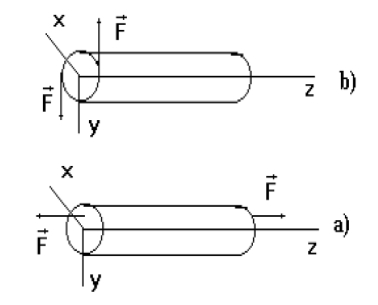
\includegraphics[width=\linewidth]{momentos.jpg}
\caption{a) Esfuerzos transversales en una barra (momento flector). b) Esfuerzos de corte (momento torsor).}
\label{fig:momentos}
\end{figure}

En particular, si se toma un segmento de la barra curvada y se considera una flexi\'on pura, el material de la parte interna de la barra estar\'a comprimido mientras que en la parte externa se encontrar\'a estirado; existiendo as\'i una capa central que no sufre deformaciones llamada superficie neutra. Las fuerzas que act\'uan por encima de la superficie neutra tienen sentido opuesto al de las fuerzas que act\'uan por debajo de dicha superficie; estos pares de fuerzas tienen un momento no nulo respecto de la superficie neutra.	Aplicando esto \'ultimo junto con la ley de Hooke y algunas consideraciones geom\'etricas a una secci\'on transversal de la barra, se obtiene la expresi\'on de la ecuaci\'on de la viga \cite{eq:vigas}:

\begin{equation}
\label{eq:viga}
M = \frac{E}{R}I
\end{equation}

donde $E$ es el m\'odulo de Young de la barra, $R$ su radio de curvatura e $I = \int_{A} h^2 dA$ el momento de inercia de la barra (siendo A el area de la secci\'on transversal elegida y h el desplazamiento vertical). \newline

Mediante la ecuaci\'on (\ref{eq:viga}) se puede determinar el apartamiento vertical de la barra de su posici\'on de equilibrio $y(x)$, debido a los pesos suspendidos de uno de sus extremos en un punto fijo $x$:

\begin{equation}
\label{eq:vigafeynman}
y(x) = -\frac{32mg}{\pi d^{4}E}(Lx^{2} - \frac{1}{3}x^{3})
\end{equation}

siendo $L$ y $d$ el largo y di\'ametro de la barra respectivamente.\newline


\subsection{M\'etodo din\'amico}

La ecuaci\'on que gobierna la evoluci\'on espacio-temporal del desplazamiento de una viga est\'a dada por \cite{eq:vigadyns}:

\begin{equation}
\label{eq:vigadyn}
\frac{\partial^4 s}{\partial x^4} + b\frac{\partial s}{\partial t} + \frac{\rho_{l}}{IE} \frac{\partial^2 s}{\partial t^2} = 0
\end{equation}

donde el t\'ermino proporcional a $\frac{\partial s}{\partial t}$ determina los efectos del amortiguamiento. Esta ecuaci\'on puede resolverse por el metodo de variables separables, obteniendo soluciones del tipo $s(x,t) = Y(t)X(x)$. \newline

La soluci\'on para $Y(t)$ resulta ser una senoidal amortiguada, con amortiguamiento $\alpha$ y frecuencia $\omega_{k}$, donde:

\begin{equation}
\label{eq:omegas}
\omega_{k} = 2\pi f_{k} = \sqrt{\frac{IE}{\rho_{l}}k^{4} - \alpha^2}
\end{equation}

siendo $\alpha = \frac{IE}{2\rho_{l}}b$ la constante de amortiguamento de la barra, $I = \frac{\pi d^4}{64}$ su momento de inercia y $\rho_{l}$ la densidad por unidad de longitud. \newline

La soluci\'on para la parte espacial es $X(x) = Acos(kx) + Bsen(kx) + Ccosh(kx) + Dsenh(kx)$; la cual junto a las condiciones de contorno (barra en voladizo) $X(0) = X'(0)$ y $X''(L) = X'''(L) = 0$ dan la siguiente ecuaci\'on para los posibles valores de $k$:

\begin{equation}
\label{eq:condiciones}
cos(kL)cosh(kL) + 1 = 0
\end{equation}

De la ecuaci\'on (\ref{eq:condiciones}) pueden obtenerse los valores de $k$:  $k_{1} = \frac{1,875}{L}$ para el modo fundamental, $k_{2} = \frac{4,694}{L}$ para el segundo modo, $k_{3} = \frac{7,855}{L}$ para el tercero.

Por cuestiones pr\'acticas al momento del c\'alculo, nos quedaremos s\'olo con $k_{1}$.


%------------------------------------------------

\section{Dispositivo experimental}

Los instrumentos de laboratorio utilizados en ambos m\'etodos fueron:
\begin{itemize}
\item 
\label{Laser} L\'aser marca Melles Griot, modelo 06DAL003 de 670 nm.
\item Espejos marca Melles Griot.
\item Pesos y soporte para pesos.
\item Barras de lat\'on y de hierro de diferentes longitudes y pesos.
\item Rendija de metal.
\item Fotodiodo marca ThorLabs, modelo DET36A/M.
\item Placa de adquisici\'on de datos marca National Instruments, modelo NIUSB-6212.
\item Computadora personal con software MATLAB para la recolecci\'on y an\'alisis de datos.
\end{itemize}

\subsection{M\'etodo est\'atico}

\subsection{M\'etodo din\'amico}

Para este m\'etodo se utiliz\'o pr\'acticamente el mismo dispositivo experimental que en el est\'atico, con la excepci\'on de que se quitaron los pesos y se utilizaron dos barras de lat\'on (diferenciandose entre s\'i por su di\'ametro, longitud y peso) y otra de hierro. En la siguiente tabla se detallan los valores tomados para cada barra:\newline

\begin{table}[H]
\centering
\caption{Di\'ametros $d$, longitudes $L$ y pesos $m$ de las tres barras utilizadas.}
\label{tab:valoresbarras}
\begin{tabular}{|c|c|c|c|}
\hline
Material & $d$ $\pm$ 0,002 & $L$ $\pm$ 0,1 & $m$ $\pm$ 0,1\\ \hline
Lat\'on & 0,471 cm & 31,02 cm & 51,22 g\\ \hline
Hierro & 0,369 cm & 36,10 cm & 36,57 g  \\ \hline
Lat\'on fino & 0,243 cm & 40,30 cm & 22,02 g \\ \hline
\end{tabular}
\end{table}


Adem\'as, se agreg\'o un fotodiodo de \ce{^{28}_{14}Si} marca ThorLabs modelo DET36A/M justo detr\'as del extremo libre de la barra para poder registrar las oscilaciones verticales de la misma. \newline
\'Este \'ultimo se conect\'o a una placa de adquisici\'on de datos marca National Instruments NIUSB-6212, y mediante un programa hecho en MATLAB se registr\'o, durante 60 segundos y a una frecuencia de 1000 Hz, la se\~nal capturada por el fotodiodo. En la Figura (\ref{fig:dispexp_dinamico}) se muestra este arreglo experimental.

\begin{figure}[H]
\includegraphics[width=\linewidth]{dispexp_dinamico.jpg}
\caption{Dispositivo experimental utilizado en el m\'etodo din\'amico. Se pueden ver los siguientes elementos: A) L\'aser, B) Barra y soporte, C) Espejos para redireccionar el haz hacia el extremo libre de la barra, D) Fotodiodo.}
\label{fig:dispexp_dinamico}
\end{figure}

Cabe destacar que, para poder estar seguros de que la frecuencia de 1000 Hz elegida para el sampleo de los datos era suficiente; se realiz\'o un breve c\'alculo a mano para obtener las frecuencias de oscilaci\'on de los tres primeros modos mediante las ecuaciones (\ref{eq:omegas}) y (\ref{eq:condiciones}), tomando $\alpha = 0$; dando como resultado valores de $f_{k} < 500$ Hz, con lo cual se satisfacieron las condiciones del teorema de Nyquist-Shannon \cite{teo:shannon}

La determinaci\'on del factor de amortiguamiento $\alpha$ se llevo a cabo mediante un ajuste sobre la se\~nal original con una forma funcional senoidal amortiguada exponencialmente.
Para calcular las frecuencias $f_{k}$, se realiz\'o un an\'alisis de Fourier sobre la se\~nal obtenida por el fotodiodo y as\'i poder obtener el valor del m\'odulo de Young $E$ mediante la ecuaci\'on (\ref{eq:omegas}) y la constante de amortiguamiento previamente calculada.

Por \'ultimo, para la barra de lat\'on fino se analiz\'o como varia la frecuencia fundamental y el factor de amortiguamiento en funci\'on de la longitud de la barra (cambiando la posici\'on del extremo fijo de la misma), partiendo de $L_{1} = 40,3 \pm 0,1$ cm, en decrementos de 4 cm, hasta $L_{6} = 20,3 \pm 0,1$ cm.



%------------------------------------------------
\section{Resultados y an\'alisis}

METODO ESTATICO


\subsection{M\'etodo din\'amico}

Con los datos obtenidos de la se\~nal enviada por el fotodiodo, se realizo un ajuste exponencial sobre la misma para poder obtener el factor de amortiguamiento $\alpha$ para las tres barras, tomando como longitud total de cada barra las detalladas en la Tabla \ref{tab:valoresbarras}. \newline

En la siguiente figura, se puede observar que la se\~nal decae en el tiempo como una sinoidal con una envolvente exponencial. Tambi\'en se puede ver que se marcaron los picos de cada m\'aximo, para luego poder obtener el factor $\alpha$ mediante el ajuste mencionado al principio.

\begin{figure}[H]
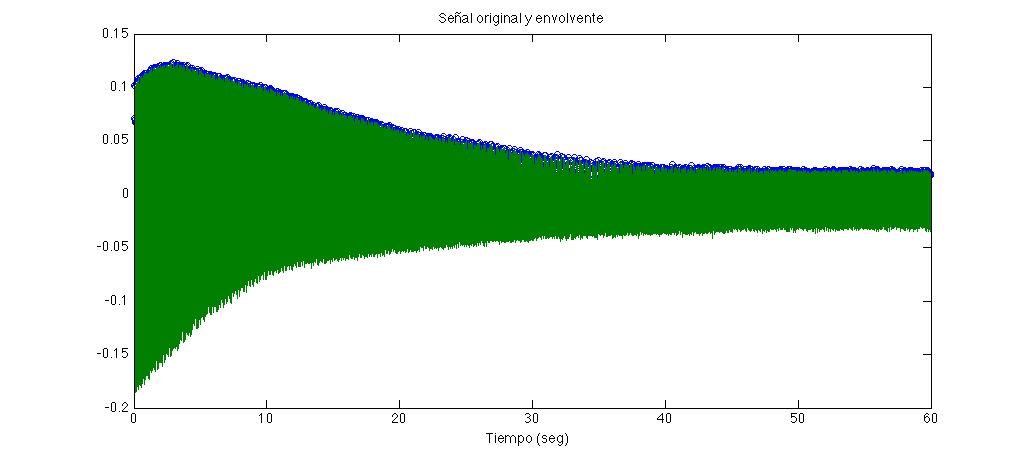
\includegraphics[width=\linewidth]{senalenvolvente.jpg}
\caption{Se\~nal obtenida para la barra de lat\'on y su envolvente.}
\label{fig:senalenvolvente}
\end{figure}

Luego, se obtuvieron las frecuencias de resonancia de cada barra mediante an\'alisis de Fourier. Como se dijo en la Introducci\'on, para la adquisici\'on de los datos se fijo un tiempo de 60 segundos y una frecuencia de sampleo de 1000 Hz. Al calcular la transformada de Fourier de la se\~nal y obtener las frecuencias, se noto que si bien aparec\'ia la fundamental y los primeros dos arm\'onicos, entre estos exist\'ian frecuencias que no correspond\'ian a modos de resonancia de la barra si no a factores tales como el efecto rebote introducido por el movimiento oscilante de la misma.

Como ejemplo, en la siguiente figura se puede ver el espectro de frecuencias de la barra de lat\'on en su longitud original $L_{1} = 31,2 \pm 0,1$ cm. Pueden apreciarse la frecuencia fundamental $f_{1} \approx 20,20$ Hz y las correspondientes al efecto de rebote ($f \approx 40,41$ Hz, etc). \newline

\begin{figure}[H]
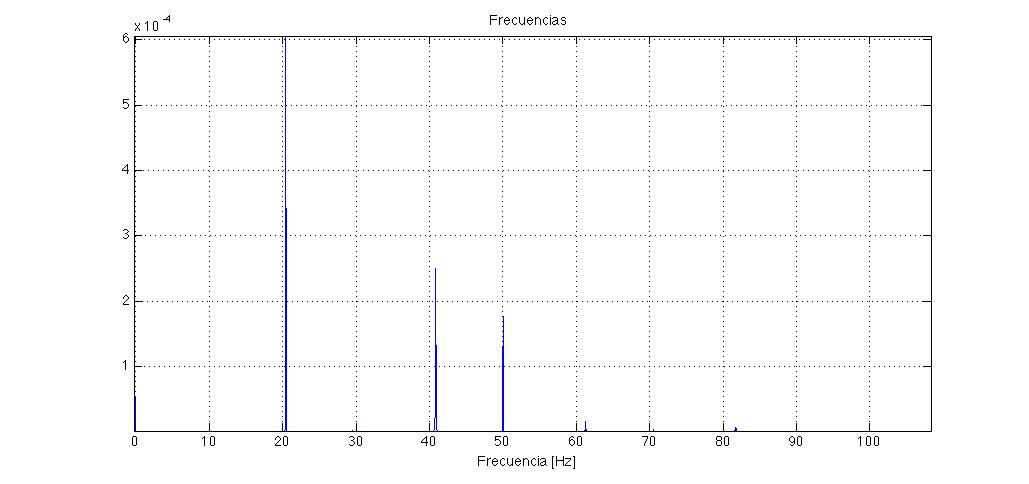
\includegraphics[width=\linewidth]{espectrolaton.jpg}
\caption{Parte del espectro de frecuencias para la barra de lat\'on. Se pueden observar la frecuencia fundamental $f_{1} \approx 20,2$ Hz y frecuencias del rebote.}
\label{fig:espectrolaton}
\end{figure}

Si bien para calcular el m\'odulo de Young solo se utiliz\'o la frecuencia del modo fundamental (y su correspondiente $k$), se pudo obtener las frecuencias del primer y segundo arm\'onico. Esto resulto mas dif\'icil de observar en los espectros debido a que los picos correspondientes a estas frecuencias era muy peque\~nos con respecto al del fundamental.\newline Siguiendo con el ejemplo de la barra de lat\'on, se calcularon dichas frecuencias mediante la ecuacion (\ref{eq:omegas}) junto con la constante de amortiguamiento $\alpha$, obteniendo los siguientes valores: $f_{1} \approx 20,20$ Hz, $f_{2} \approx 122,50$ Hz y $f_{3} \approx 354$ Hz. \newline

\begin{figure}[H]
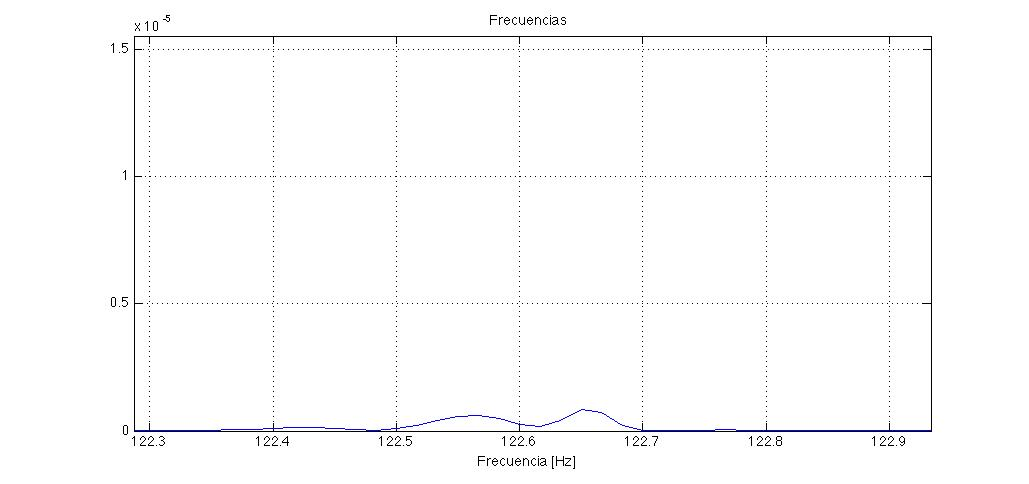
\includegraphics[width=\linewidth]{espectrolatonarmonico.jpg}
\caption{Parte del espectro de frecuencias para la barra de lat\'on. Al aumentar el zoom en el espectro, se puede observar el primer arm\'onico con frecuencia $f_{2} \approx 122,50$ Hz, con una amplitud muy peque\~na en relaci\'on a $f_{1} \approx 20,20$ Hz}
\label{fig:espectrolatonarmonico}
\end{figure}


En la siguiente tabla se detallan los valores de la frecuencia fundamental $f_{1}$ para las tres barras, utilizando $k_{1} = \frac{1,875}{L}$ y la constante de amortiguamiento $\alpha$ correspondiente a cada una con un nivel de confianza del 95\%:


\begin{table}[H]
\centering
\caption{Frecuencias fundamentales y constantes de amortiguamiento para cada barra.}
\label{tab:fya_barras}
\begin{tabular}{|c|c|c|}
\hline
Material & $f_{1}$ (Hz) & $\alpha$ (Hz) \\ \hline
Lat\'on & 20,20 & 0,0335 $\pm$ 0,0009\\ \hline
Hierro & 21,78 & 0,1343 $\pm$ 0,0009  \\ \hline
Lat\'on fino & 8,25 & 0,0190 $\pm$ 0,0009\\ \hline
\end{tabular}
\end{table}


Adem\'as, se calcul\'o la densidad lineal de cada barra a partir de su peso y longitud, as\'i como tambi\'en el momento de inercia $I$ de acuerdo a la geometr\'ia cil\'indrica de las mismas. Estos datos se encuentran en la siguiente tabla :

\begin{table}[H]
\centering
\caption{Valores de longitud $L$, densidad lineal $\rho_{l}$ y momento de inercia $I$ para cada barra.}
\label{tab:params_barras}
\begin{tabular}{|c|c|c|c|}
\hline
Material & $L$ (cm) & $\rho_{l}$ (g/cm) & $I$ $(cm^{4})$\\ \hline
Lat\'on & 31,2 $\pm$ 0,1 & 1,64 $\pm$ 0,01 & 0,0024 $\pm$ 0,0001\\ \hline
Hierro & 36,1 $\pm$ 0,1 & 1,01 $\pm$ 0,01 & 0,0009 $\pm$ 0,0001\\ \hline
Lat\'on fino & 40,3 $\pm$ 0,1 & 0,55 $\pm$ 0,01 & 0,0002 $\pm$ 0,0001\\ \hline
\end{tabular}
\end{table}


Luego, mediante la ecuaci\'on (\ref{eq:omegas}) y los datos de las Tablas \ref{tab:fya_barras} y \ref{tab:params_barras}, se obtuvieron los valores de los m\'odulos de Young de cada una de las tres barras estudiadas:

\begin{table}[H]
\centering
\caption{M\'odulo de Young $E$ de cada una de las tres barras. Se puede observar que corresponden al orden de los valores te\'oricos dados por \cite{teo:ashby}}

\label{tab:young_barras}
\begin{tabular}{|c|c|}
\hline
Material & $E$ (Pa)\\ \hline
Lat\'on & $8,44 * 10^{10}$ $\pm$ 0,1\\ \hline
Hierro & $2,89 * 10^{11}$ $\pm$ 0,1\\ \hline
Lat\'on fino & $1,58 * 10^{11}$ $\pm$ 0,1\\ \hline
\end{tabular}
\end{table}

Para finalizar, se analiz\'o como var\'ia la frecuencia fundamental y el factor de amortiguamiento en funci\'on de la longitud de la barra de lat\'on fino, con los par\'ametros mencionados al final de  la secci\'on 2.2

\begin{figure}[H]
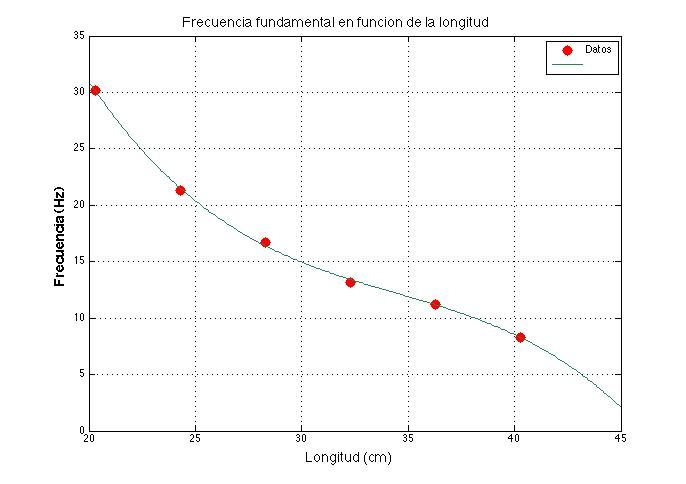
\includegraphics[width=\linewidth]{fvsl.jpg}
\caption{Frecuencias fundamentales de la barra de lat\'on fino en funci\'on de su longitud.}
\label{fig:fvsl}
\end{figure}

\begin{figure}[H]
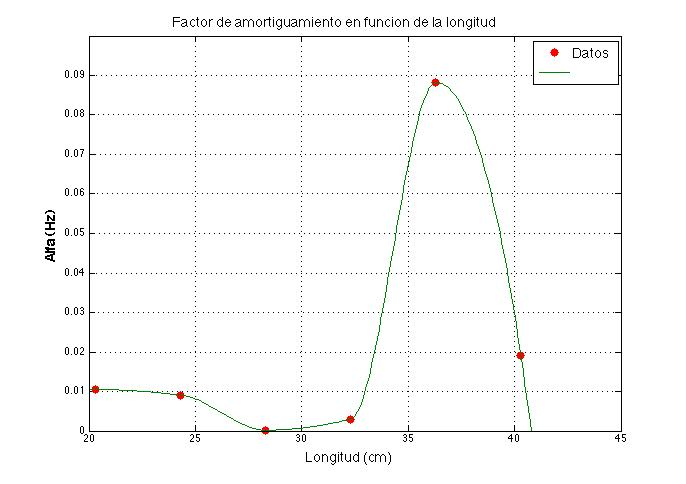
\includegraphics[width=\linewidth]{avsl.jpg}
\caption{Factor de amortiguamiento de la barra de lat\'on fino en funci\'on de su longitud.}
\label{fig:avsl}
\end{figure}

Puede apreciarse en los gr\'aficos que la frecuencia fundamental va aumentando al disminuir la longitud; dado que a menor longitud el material es mas r\'igido por lo tanto oscilar\'a a mayor frecuencia, destacando desproporcionadamente a la fundamental sobre los arm\'onicos, siendo estos \'ultimos pr\'acticamente imperceptibles en este caso. \newline

Por el contrario, si observamos el gr\'afico para el factor de amortiguamiento $\alpha$ en funci\'on de la longitud $L$; se puede destacar que para $L < L_{4} = 28,3$ cm, $\alpha$ decrece por lo tanto la barra oscilar\'a durante m\'as tiempo ocasionando que el espectro de frecuencias sea m\'as parejo, con el costo de introducir una mayor cantidad de frecuencias no deseadas.
A partir de $L > L_{4} = 28,3$ cm, $\alpha$ vuelve a crecer hasta alcanzar un valor m\'aximo en $L_{2} = 36,3$.

Cabe aclarar que, para esta parte de la experiencia, se intent\'o tomar longitudes m\'as cortas a $L_{6} = 20,3$ cm, pero observamos que los datos recolectados eran muy similares a una barra en reposo, por lo tanto no generaban valores significativos de $f$ y $\alpha$.

%------------------------------------------------

\section{Conclusiones}

Comparando los valores obtenidos de la resistencia en los distintos ajustes (lineal, cuadr\'atico y c\'ubico), se encontr\'o que el modelo que mejor explica los datos recolectados es el cuadr\'atico con todos sus par\'ametros libres ($R^2$ = 0,99999), esto quiere decir que este modelo explica en gran medida los datos obtenidos. Su F-valor de 1E6 muestra que es muy improbable que este polinomio ajustara de forma aleatoria. Al observar los residuos de este ajuste, se not\'o que parecen ser independientes de la intensidad, indicando que el ajuste realizado es un buen modelo para caracterizar el sistema.
\par

En el ajuste lineal, es posible notar una fuerte dependencia, similar a una cuadr\'atica, de los residuos en funci\'on de la intensidad. Debido a esto, se podr\'ia considerar que en el caso de la l\'ampara incandescente, la ecuaci\'on (\ref{eq:ohm2}) no es aplicable directamente, sino que se tuvo que considerar el efecto de la temperatura.

El ultimo ajuste realizado fue el c\'ubico, que coincidi\'o en gran parte con los valores dados por el cuadr\'atico ($R^2$ y residuos). Sin embargo, al observar los T-valores para los distintos par\'ametros, estos fueron considerablemente peores que en el anterior. En particular para el coeficiente c\'ubico se observa un bajo T-valor, lo que mostr\'o que este tercer par\'ametro tiene una baja significancia.

%----------------------------------------------------------------------------------------
%	REFERENCE LIST
%----------------------------------------------------------------------------------------

\begin{thebibliography}{99} % Bibliography - this is intentionally simple in this template


\bibitem{eq:leyhooke} M. Alonso, E. J. Finn, \textit{F\'isica - Vol. 1}, Editorial Addison-Wesley Iberoamericana (1986), p\'ag. 363

\bibitem{eq:vigas} W. Seto, \textit{Theory and problems of mechanical vibrations}, Editorial McGraw Hill, 2da edici\'on, Barcelona (1971), Cap. 9
\bibitem{eq:vigadyns} S. C. Hunter, \textit{Mechanics of continuous media}, John Wiley and Sons (1986)
\bibitem{teo:shannon} S. Ghosh, \textit{Signals and Systems}, Editorial Pearson Education, India (2006), Cap. 3
\bibitem{teo:ashby} M. F. Ashby, D. R. H. Jones, \textit{Materiales para Ingenier\'ia 1 - Introducci\'on a las propiedades, las aplicaciones y el dise\~no}, Editorial Revert\'e S.A., edici\'on en espa\~nol, Barcelona (2008), p\'ag. 39

 
\end{thebibliography}


%----------------------------------------------------------------------------------------

\end{document}